\documentclass[a4paper, 14pt]{extarticle}

% Поля
%--------------------------------------
\usepackage{geometry}
\geometry{a4paper,tmargin=2cm,bmargin=2cm,lmargin=3cm,rmargin=1cm}
%--------------------------------------


%Russian-specific packages
%--------------------------------------
\usepackage[T2A]{fontenc}
\usepackage[utf8]{inputenc} 
\usepackage[english, main=russian]{babel}
%--------------------------------------

\usepackage{textcomp}

% Красная строка
%--------------------------------------
\usepackage{indentfirst}               
%--------------------------------------             


%Graphics
%--------------------------------------
\usepackage{graphicx}
\graphicspath{ {./images/} }
\usepackage{wrapfig}
%--------------------------------------

% Полуторный интервал
%--------------------------------------
\linespread{1.3}                    
%--------------------------------------

%Выравнивание и переносы
%--------------------------------------
% Избавляемся от переполнений
\sloppy
% Запрещаем разрыв страницы после первой строки абзаца
\clubpenalty=10000
% Запрещаем разрыв страницы после последней строки абзаца
\widowpenalty=10000
%--------------------------------------

%Списки
\usepackage{enumitem}

%Подписи
\usepackage{caption} 

%Гиперссылки
\usepackage{hyperref}

\hypersetup {
	unicode=true
}

%Рисунки
%--------------------------------------
\DeclareCaptionLabelSeparator*{emdash}{~--- }
\captionsetup[figure]{labelsep=emdash,font=onehalfspacing,position=bottom}
%--------------------------------------

\usepackage{tempora}

%Листинги
%--------------------------------------
\usepackage{listings}
\lstset{
	basicstyle=\ttfamily\footnotesize, 
	%basicstyle=\footnotesize\AnkaCoder,        % the size of the fonts that are used for the code
	breakatwhitespace=false,         % sets if automatic breaks shoulbd only happen at whitespace
	breaklines=true,                 % sets automatic line breaking
	captionpos=t,                    % sets the caption-position to bottom
	inputencoding=utf8,
	frame=single,                    % adds a frame around the code
	keepspaces=true,                 % keeps spaces in text, useful for keeping indentation of code (possibly needs columns=flexible)
	keywordstyle=\bf,       % keyword style
	numbers=left,                    % where to put the line-numbers; possible values are (none, left, right)
	numbersep=5pt,                   % how far the line-numbers are from the code
	xleftmargin=25pt,
	xrightmargin=25pt,
	showspaces=false,                % show spaces everywhere adding particular underscores; it overrides 'showstringspaces'
	showstringspaces=false,          % underline spaces within strings only
	showtabs=false,                  % show tabs within strings adding particular underscores
	stepnumber=1,                    % the step between two line-numbers. If it's 1, each line will be numbered
	tabsize=2,                       % sets default tabsize to 8 spaces
	title=\lstname                   % show the filename of files included with \lstinputlisting; also try caption instead of title
}
%--------------------------------------

%%% Математические пакеты %%%
%--------------------------------------
\usepackage{amsthm,amsfonts,amsmath,amssymb,amscd}  % Математические дополнения от AMS
\usepackage{mathtools}                              % Добавляет окружение multlined
\usepackage[perpage]{footmisc}
%--------------------------------------

%--------------------------------------
%			НАЧАЛО ДОКУМЕНТА
%--------------------------------------

\begin{document}
	
	%--------------------------------------
	%			ТИТУЛЬНЫЙ ЛИСТ
	%--------------------------------------
	\begin{titlepage}
		\thispagestyle{empty}
		\newpage
		
		
		%Шапка титульного листа
		%--------------------------------------
		\vspace*{-60pt}
		\hspace{-65pt}
		\begin{minipage}{0.3\textwidth}
			\hspace*{-20pt}\centering
			
\includegraphics[width=\textwidth]{emblem}
		\end{minipage}
		\begin{minipage}{0.67\textwidth}\small \textbf{
				\vspace*{-0.7ex}
				\hspace*{-6pt}\centerline{Министерство науки и высшего образования Российской Федерации}
				\vspace*{-0.7ex}
				\centerline{Федеральное государственное бюджетное образовательное учреждение }
				\vspace*{-0.7ex}
				\centerline{высшего образования}
				\vspace*{-0.7ex}
				\centerline{<<Московский государственный технический университет}
				\vspace*{-0.7ex}
				\centerline{имени Н.Э. Баумана}
				\vspace*{-0.7ex}
				\centerline{(национальный исследовательский университет)>>}
				\vspace*{-0.7ex}
				\centerline{(МГТУ им. Н.Э. Баумана)}}
		\end{minipage}
		%--------------------------------------
		
		%Полосы
		%--------------------------------------
		\vspace{-25pt}
		\hspace{-35pt}\rule{\textwidth}{2.3pt}
		
		\vspace*{-20.3pt}
		\hspace{-35pt}\rule{\textwidth}{0.4pt}
		%--------------------------------------
		
		\vspace{1.5ex}
		\hspace{-35pt} \noindent \small ФАКУЛЬТЕТ\hspace{80pt} <<Информатика и системы управления>>
		
		\vspace*{-16pt}
		\hspace{47pt}\rule{0.83\textwidth}{0.4pt}
		
		\vspace{0.5ex}
		\hspace{-35pt} \noindent \small КАФЕДРА\hspace{50pt} <<Теоретическая информатика и компьютерные технологии>>
		
		\vspace*{-16pt}
		\hspace{30pt}\rule{0.866\textwidth}{0.4pt}
		
		\vspace{11em}
		
		\begin{center}
			\Large {\bf Лабораторная работа № 6} \\ 
			\large {\bf по курсу <<Языки и методы программирования>>} \\
			\large <<Программа с графическим пользовательским интерфейсом>> 
		\end{center}\normalsize
		
		\vspace{8em}
		
		
		\begin{flushright}
			{Студент группы ИУ9-22Б Тараканов В. Д. \hspace*{15pt}\\ 
				\vspace{2ex}
				Преподаватель Посевин Д. П.\hspace*{15pt}}
		\end{flushright}
		
		\bigskip
		
		\vfill
		
		
		\begin{center}
			\textsl{Москва 2024}
		\end{center}
	\end{titlepage}
	%--------------------------------------
	%		КОНЕЦ ТИТУЛЬНОГО ЛИСТА
	%--------------------------------------
	
	\renewcommand{\ttdefault}{pcr}
	
	\setlength{\tabcolsep}{3pt}
	\newpage
	\setcounter{page}{2}
	
	\section{Задание}\label{Sect::task}
	
	Круг диаметра d, разбитый на n равных секторов, закрашенных случайными цветами.
	
	\section{Результаты}\label{Sect::res}
	\begin{figure}[!htb]
		\begin{lstlisting}[language={},caption={Класс PictureForm},label={lst:code1}]
		import javax.swing.*;
		import javax.swing.event.ChangeEvent;
		import javax.swing.event.ChangeListener;
		
		public class PictureForm {
			private JPanel panel1;
			private JSpinner radiusSpiner;
			private JSpinner sectorsSpiner;
			private CanvasPanel canvasPanel1;
			
			
			public PictureForm(){
				radiusSpiner.setValue(200);
				
				radiusSpiner.addChangeListener(new ChangeListener() {
					@Override
					public void stateChanged(ChangeEvent changeEvent) {
						int radius = (int)radiusSpiner.getValue();
						canvasPanel1.setRadius(radius);
					}
				});
				sectorsSpiner.addChangeListener(new ChangeListener() {
					@Override
					public void stateChanged(ChangeEvent changeEvent) {
						int sectors = (int)sectorsSpiner.getValue();
						canvasPanel1.setSectors(sectors);
					}
				});
			}
			public static void main(String[] args) {
				JFrame frame = new JFrame("PictureForm");
				frame.setContentPane(new PictureForm().panel1);
				frame.setDefaultCloseOperation(JFrame.EXIT_ON_CLOSE);
				frame.pack();
				frame.setSize(800,600);
				frame.setVisible(true);
			}	
		}
		\end{lstlisting}
	\end{figure}
	
	\newpage
	
	\begin{figure}[!htb]
		\begin{lstlisting}[language={},caption={Класс CanvasPanel},label={lst:code2}]
			import javax.swing.*;
			import java.awt.*;
			import java.awt.geom.Line2D;
			import java.util.Random;
			
			public class CanvasPanel extends JPanel {
				private int radius = 20;
				Random random = new Random();
				private int x;
				private int y;
				private int sectors = 0;
				public void setRadius(int r) {
					radius = r;
					x = 10+radius/2;
					y = 10+radius/2;
					repaint();
				}
				public void setSectors(int s){
					sectors = s;
					repaint();
				}
				protected void paintComponent(Graphics g) {
					super.paintComponent(g);
					
					Graphics2D g2 = (Graphics2D) g;
					g2.setRenderingHint(RenderingHints.KEY_ANTIALIASING,
					RenderingHints.VALUE_ANTIALIAS_ON);
					g2.setColor(Color.RED);
					g2.drawOval(10,10,radius,radius);
					for(int i = 0;i<sectors;i++){
						Color randomColor = new Color(random.nextInt(256), random.nextInt(256), random.nextInt(256));
						g.setColor(randomColor);
						int startAngle = i * 360 / sectors;
						int angle = 360 / sectors+1;
						
						g.fillArc(x - radius/2, y - radius/2, radius, radius, startAngle, angle);
					}
					
				}
			}
			
			\end{lstlisting}
		\end{figure}
		
		Результат запуска представлен на рисунках~\ref{fig:img1}--~\ref{fig:img2}.
		
		\begin{figure}[!htb]
			\centering
			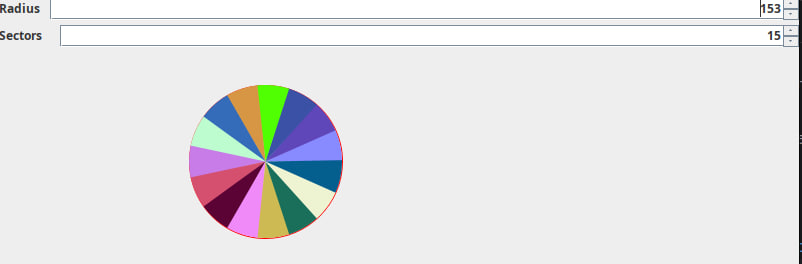
\includegraphics[width=0.5\textwidth]{img1}
			\caption{Результат}
			\label{fig:img1}
		\end{figure}
		\begin{figure}[!htb]
			\centering
			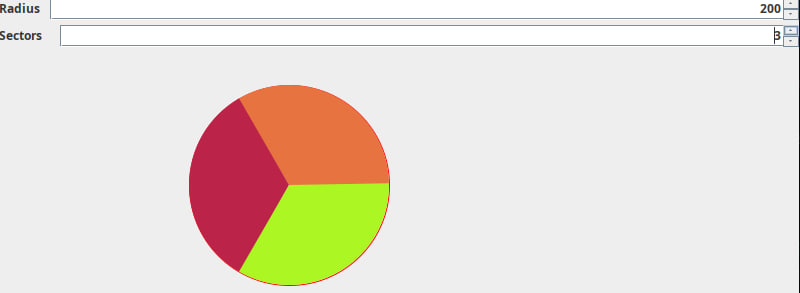
\includegraphics[width=0.5\textwidth]{img2}
			\caption{Результат}
			\label{fig:img2}
		\end{figure}
		
	\end{document}
